\documentclass[12pt]{article}

\usepackage{amsmath}
\usepackage[utf8]{inputenc}
\usepackage[T1]{fontenc}
\usepackage[magyar]{babel}
\usepackage{graphicx}
\usepackage{float}
\usepackage[paper=a4paper,margin=1in]{geometry}

\usepackage{siunitx}
%%\title{%
%%  Kondenzált anyagok fizikája \\
%%  \large 1. Gyakorlat}
%%\author{}  
%%\maketitle


\begin{document}


\centerline{
\textsc{\Large{ Kondenzált anyagok fizikája}}
}
\centerline{ 
\textsc{\large{3. Gyakorlat}}
}
\vspace{10mm}

\textbf{Gy1.} Határozzuk meg az FCC rács szoros pakolású síkjának (csúszósíkjának) Miller-indexeit!
\\

\textbf{Gy2.} Rajzoljunk be a három üres koordináta-rendszerbe egy-egy olyan rácssíkot, amelynek helyzetét a koordináta-rendszer alatt található Miller-indexek írják le, valamint adjuk meg a három másik ábrán berajzolt síkok Miller-indexeit. (A felülvonás negatív Miller-indexet jelent.)
\begin{figure}[h!]
\begin{center}
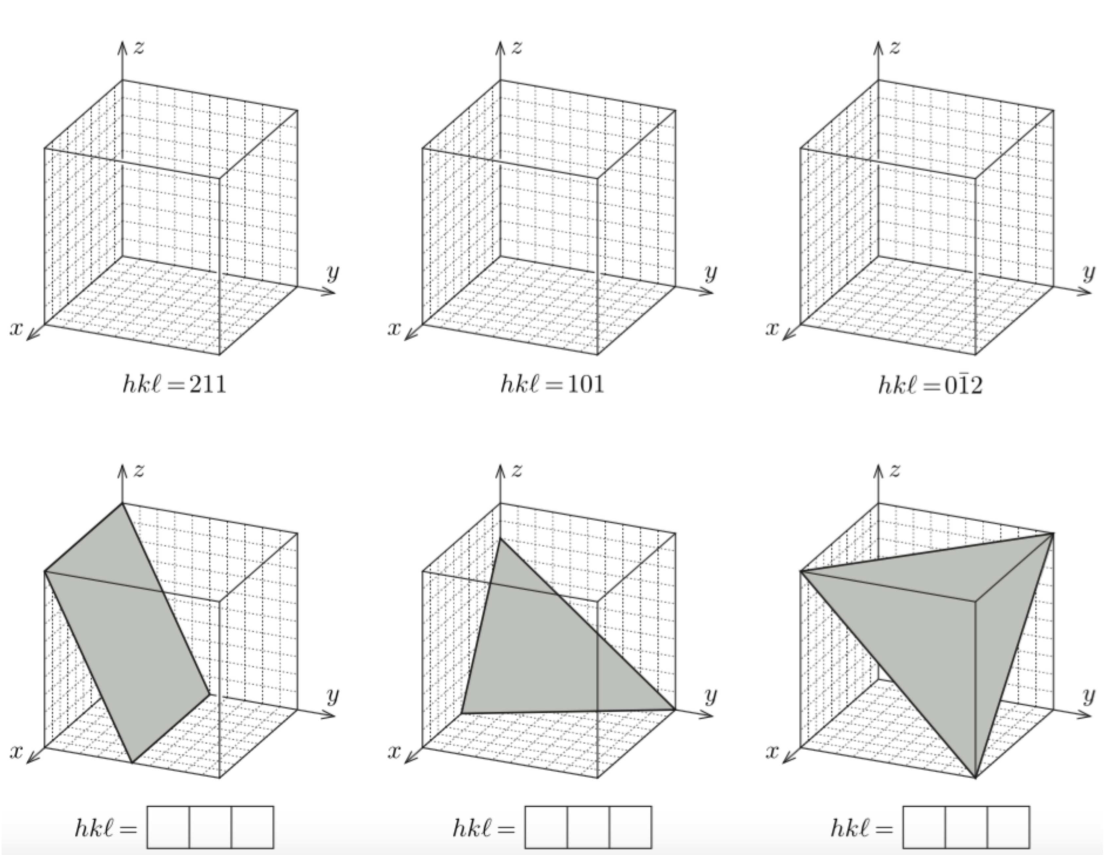
\includegraphics[height=10cm]{../images/kristalysikok.png} 
\end{center}
\end{figure}

\textbf{Gy3.} Határozzuk meg az alábbi ábrán látható kristálysík Miller-indexeit!
\begin{figure}[h!]
\begin{center}
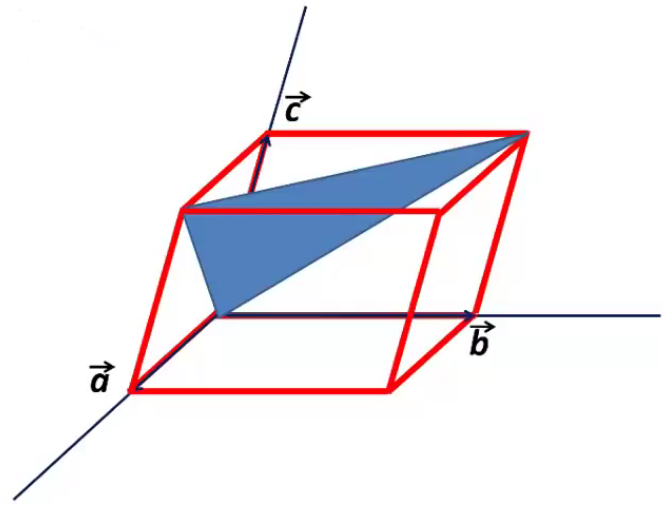
\includegraphics[height=5cm]{../images/ferdeszogu-11m1.png} 
\end{center}
\end{figure}
\\

\textbf{Gy4.} Határozzuk meg az FCC kristályrácsú nikkel azon síkseregének h, k, l indexeit, melyre a síkok közötti távolság d = 1.246 Å. A rácsállandó a = 3.524 Å.
\\

\textbf{Gy5.} Vázlatosan rajzoljuk fel egy köbös elemi cellában a következő kristálysíkokat: (111), (210),
és (003)

\end{document}